% !TEX encoding = UTF-8 Unicode
\documentclass[a4paper]{article}

\usepackage[utf8]{inputenc}
\usepackage{erk}
\usepackage{times}
\usepackage{wrapfig}
\usepackage{graphicx}
\usepackage{xcolor}
\usepackage[top=22.5mm, bottom=22.5mm, left=22.5mm, right=22.5mm]{geometry}
\usepackage{float}  % add this in your preamble (before \begin{document})


\usepackage[slovene,english]{babel}

% to-do command
\newcommand\todocomment[1]{\textcolor{red}{||\\ #1\\||}}


% local definitions
\def\footnotemark{}%  to avoid footnote on cover page

\begin{document}
%make title
\title{Utilizing Convolution for Obstacle Avoidance during Robotic Manipulator Movement}

\author{Jakob Baumgartner$^{1}$, Gregor Klančar$^{2}$} % use ^1, ^2 for author(s) from different institutions

\affiliation{$^{1}$Fakulteta za Elektrotehniko, Tržaška cesta 25, 1000 Ljubljana\\}

\email{E-pošta: jakob.baumgartner@fe.uni-lj.si}

\maketitle

%\thispagestyle{empty}

\begin{abstract}{Abstract}
\todocomment{ADD}
\end{abstract}


\selectlanguage{slovene}

\section{Introduction }

Robotic manipulators, specifically those with a high degree of freedom (DOF), possess a crucial characteristic known as kinematic redundancy. Kinematic redundancy refers to having more joints (i.e., degrees of freedom - DOF) than required to perform a task, thus allowing the robot to adopt multiple configurations to accomplish the same end-effector position and orientation. This redundancy provides a considerable advantage, making it possible for manipulators to optimize movement according to different criteria, such as energy efficiency, obstacle avoidance, or joint limit avoidance.

In this research, we specifically consider a 7-DOF Panda Emika manipulator. When controlling both the position and orientation of the end-effector in a 3D space, which requires six degrees of freedom (three for position and three for orientation), a 7-DOF manipulator such as the Panda Emika has one redundant degree. However, when controlling only the position, which requires three degrees of freedom, the manipulator possesses four redundant degrees. This redundancy grants the manipulator an essential characteristic: an infinite number of possible joint configurations to reach a specific end-effector (EE) point in space.

When dealing with redundant manipulators, task prioritization is crucial. In our approach, we distinguish between primary and secondary tasks. The primary task of the manipulator is usually defined as reaching a desired EE position and orientation or as following a trajectory made out of such points. In this work we instead use APF (Artificial Potential Field), to guide the EE towards the goal position, while avoiding the obstacles in the path of the EE. Operating in a real-world environment often requires considering secondary tasks, such as real-time obstacle avoidance, to ensure safe and uninterrupted operation of the manipulator.

\todocomment{IMAGE OF ROBOT}

This paper proposes a novel method for real-time obstacle avoidance in the Panda Emika 7-DOF manipulator. We use an obstacle grid combined with convolution techniques to assign avoidance directions to each manipulator segment, ensuring efficient and safe maneuvering within complex environments. 


\todocomment{Dodaj opis poglavij.}

\section{Background and Related Work}

%The execution of the secondary task of obstacle avoidance necessitates an understanding of the spatial relationship between the manipulator and surrounding obstacles, usually quantified as a distance or interpreted as a repulsive force. By conceptualizing obstacles as sources of repulsive forces, the manipulator can be guided away from potential collisions, akin to how two magnets of the same polarity repel each other.
%
%Two commonly employed methods for obstacle avoidance include potential field methods and artificial neural networks. In potential field methods, the robot and obstacles are treated as charged entities. The robot is attracted to the target (goal) while being repelled by obstacles, resulting in a potential field. The robot navigates this field, moving along the path of steepest descent. While this method is intuitive and relatively easy to implement, it can sometimes result in local minima problems where the robot gets stuck in a position that is not the target but cannot find a path due to the repelling obstacles.
%
%Artificial neural networks (ANNs) are another prevalent approach, offering potential solutions to the local minima problem. By learning to map sensor readings to appropriate actions, ANNs can be trained to successfully navigate complex environments. However, they require extensive training and can be computically intensive.
%
%Our proposed approach seeks to combine the strengths of these methods, utilizing the obstacle grid and convolution techniques to efficiently calculate repulsive forces, thus enabling real-time obstacle avoidance while mitigating issues commonly associated with traditional methods.

The execution of the secondary task of obstacle avoidance necessitates an understanding of the spatial relationship between the manipulator and surrounding obstacles, usually quantified as a distance or interpreted as a repulsive force. By conceptualizing obstacles as sources of repulsive forces, the manipulator can be guided away from potential collisions, akin to how two magnets of the same polarity repel each other.

Two commonly employed methods for obstacle avoidance include potential field methods and artificial neural networks. In potential field methods, the robot and obstacles are treated as charged entities. The robot is attracted to the target (goal) while being repelled by obstacles, resulting in a potential field. The robot navigates this field, moving along the path of steepest descent. While this method is intuitive and relatively easy to implement, it can sometimes result in local minima problems where the robot gets stuck in a position that is not the target but cannot find a path due to the repelling obstacles.

Artificial neural networks (ANNs) are another prevalent approach, offering potential solutions to the local minima problem. By learning to map sensor readings to appropriate actions, ANNs can be trained to successfully navigate complex environments. However, they require extensive training and can be computically intensive.

An advanced version of ANNs in the context of 3D obstacle detection and avoidance is the use of 3D Convolutional Neural Networks (3D-CNNs). While not strictly a path planning method, 3D-CNNs can be trained to recognize obstacles and free space in 3D occupancy data. The convolutional layers in the network can learn spatial hierarchies and structures, and the final layers can output a direction or action to take. These methods, although effective, require extensive training data and computational resources, however it is capable to recognizing and avoiding some local minima. 

The Vector Field Histogram (VFH) method presents another approach. This method uses a 2D histogram grid as a spatial representation of the environment. The histogram cells are updated based on the proximity and angle of obstacles. Then a primary polar histogram is calculated from the grid cells, leading to a candidate valley for navigation. While originally developed for 2D, this method was later extended to 3D as VFH+.

Our proposed approach uses a 3D occupancy or voxel grid and 3D directional kernels, akin to Sobel filters, to perform kernel convolution and calculate the direction in which to move the robot arm to avoid obstacles. This method marries the benefits of convolutional approaches with the intuitive spatial reasoning provided by a voxel grid representation.

The primary strength of this method is its ability to swiftly calculate directional guidance for the robot arm in real-time. By using a voxel grid, we can efficiently represent the 3D environment, and the use of 3D directional kernels allows for robust calculations of obstacle proximity and directions of free space. This is beneficial in dynamic environments where quick responses are required. Moreover, this approach does not require extensive training as with neural networks, making it easier to deploy in new environments. 

\todocomment{Preveri pravilnost informacij, dodaj vire, ki potrjujejo informacije.}

\todocomment{preveri podobnost naše metode z metodo: Vector Field Histogram (VFH) }

\section{Methodology }

\subsection{Kinematics}

The manipulation capabilities of a robot are fundamentally determined by its kinematics, the mathematical description of motion without considering the forces that cause it. In our experiments, we employed a 7 degree-of-freedom (DOF) robot. The seven joints provide a high level of versatility, enabling the robot to move and orient its end-effector in a broad range of positions and directions. To calculate the movements and positions of the robot, we use both geometric and differential kinematics.

Geometric kinematics (also known as forward and inverse kinematics) focuses on the relationship between joint angles and the position and orientation of the end-effector. Forward kinematics involves calculating the position and orientation of the end-effector given the joint angles, while inverse kinematics is the process of determining the joint angles for a desired end-effector position and orientation. In the case or redundant manipulator, there isn't an unique mapping from EE coordinates to the joint coordinates. as there are exist an infinite number of different joint angles that can map to the same EE position.

Differential kinematics, also known as the Jacobian analysis, forms the foundation of robot velocity analysis. The Jacobian matrix, often represented as $J$, encapsulates the relationship between the joint velocities and the end-effector linear and angular velocities. It's derived from the partial derivatives of the forward kinematics.

The Jacobian matrix is a key element in the control of robotic manipulators. It can also be used for computing the inverse kinematics problem. However, for a 7-DOF manipulator, the Jacobian matrix is not square and its inverse does not exist in a traditional sense. In such cases, we resort to the pseudo-inverse of the Jacobian, calculated using the Moore-Penrose method. The Moore-Penrose pseudo-inverse, denoted as $J^+$, provides an approximation of the inverse for non-square matrices. 
    
The null space of the Jacobian corresponds to those joint motions which produce no movement in the end-effector. The primary task for our robot is the desired end-effector movement. The secondary task of obstacle avoidance in our research takes advantage of this null-space motion. Our method applies a repulsive velocity from detected obstacles in the environment. We calculate this velocities at certain points that are positioned on the manipulator arm segments. The robot arm is thus able to carry out the primary task while simultaneously avoiding obstacles by appropriately utilizing its redundant DOF.

\todocomment{probably needs shortening \\
			 add equations}

\subsection{Obstacle Grid}

In order to safely and efficiently navigate a robot through a complex environment, it is essential to have an appropriate representation of the robots work space. In our approach, we achieve 3D spatial understanding of the robot's surrounding environment by employing an obstacles grid, a method that transforms the environment into a three-dimensional grid of voxels (volumetric pixels).

Each voxel within this grid corresponds to a specific volume in real-world space and contains information about the occupancy of that volume. This provides a structured and spatially efficient representation of the 3D environment, including the locations and extents of any obstacles present. This 3D voxel grid can be built from sensor data, such as that obtained from a LiDAR, 3D camera, or depth sensor. Each reading from the sensor provides a point in 3D space, and these points are used to update the occupancy probability of the corresponding voxels in the grid.


\subsection{Avoidance velocities}

In our approach to robot arm obstacle avoidance, we apply a method of kernel convolution in conjunction with geometric transformations. This methodology allows us to calculate the necessary avoidance velocities for specific points of interest on the manipulator.

The process initiates with kinematic transformations which are used to map the points of interest from the robot's configuration space to the cartesian space and than onto the 3D voxel grid. These points, strategically placed on the manipulator, serve to evaluate potential collision threats with obstacles and subsequently assist in computing the necessary obstacle avoidance velocities.

Once the mapping of these points to the voxel grid is completed, we proceed to employ a specialized kernel convolution method. This method is tailored to calculate the constituent parts of the avoidance velocity vector in the Cartesian space, specifically for the x, y, and z directions. For each of these directions, we apply a separate 3D convolutional kernel.

For each direction, we utilize its corresponding kernel and extract a segment of the obstacle grid of matching size, centered at the point of interest. This leads to two equivalent-sized 3D matrices - one from the obstacle grid and the other being the kernel. We then conduct an element-wise multiplication operation between these matrices, summing the resulting values. The result of this operation provides us with the avoidance velocity in each respective direction. Through this approach, we can dynamically adjust the robot's trajectory to effectively avoid obstacles.

\subsection{Kernel Convolution}

Our convolutional kernels are essentially discrete differential operators in 3D space, and their design reflects this. These kernels bear a resemblance to the Sobel kernels, which are widely used in computer vision for edge detection and approximation of spatial derivatives. Each kernel has a primary axis aligned with the direction in which the avoidance velocity is being calculated, with the other two axes orthogonal to it. The kernel values along the primary axis exhibit a symmetric pattern: the highest value lies in the center of the kernel, with the absolute values decreasing uniformly on either side, with negative polarity on one side. This decrease simulates the derivative-like behavior of the kernel.

\begin{figure}[H]
	\centering
	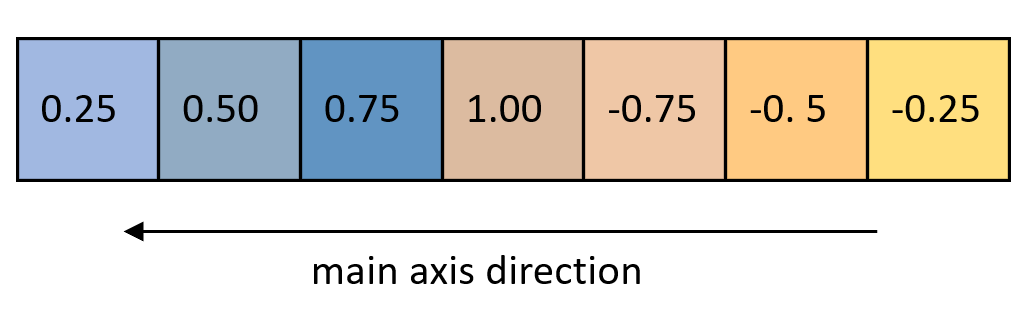
\includegraphics[width=0.85\linewidth]{kernel-mainvalues-colored.png}
	\caption{The kernel values along the primary axis exhibit a pattern of symmetrical distribution with negative polarity on one side.} 
	\label{Kernel main axis}
\end{figure}

Contrary to the design of a classical Sobel operator, our custom kernels don't contain zeroes along the primary axis. Instead, we assign the maximum kernel values along this line. This choice is specifically designed to meet our goal of obstacle avoidance. By doing so, when our points of interest on the robot manipulator coincide with an obstacle - effectively being 'right on top' of the obstacle in the voxel grid - the convolution operation yields a maximal repulsive velocity. This encourages the robot to move away from the obstacle and ensures safer navigation in the presence of potential collisions.

\begin{figure}[H]
	\centering
	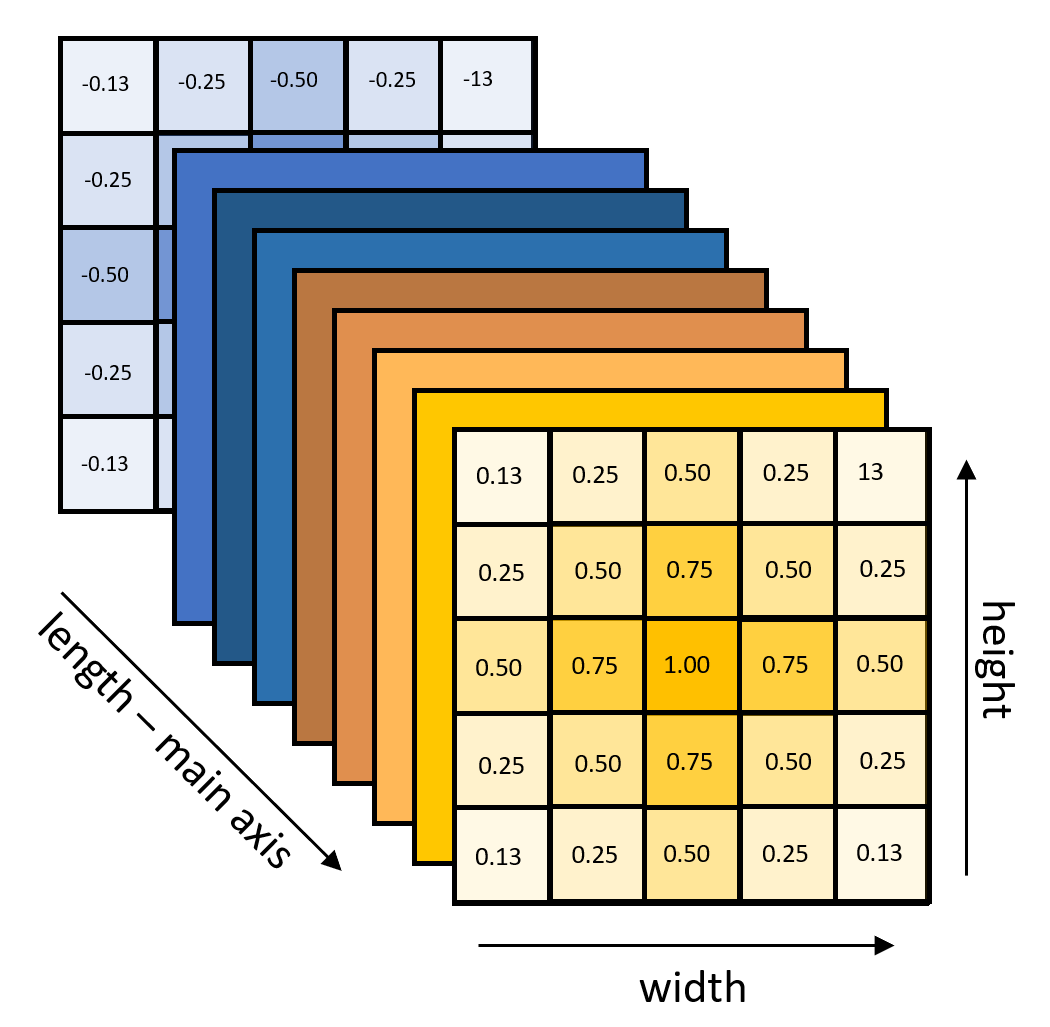
\includegraphics[width=0.85\linewidth]{kernel-matrix.png}
	\caption{In most instances, an equal width and height around the primary axis are desired, creating a symmetrical detection area.} 
	\label{Kernel matrix}
\end{figure}

\todocomment{while not the most important fix, currently values in matrix don't follow values used in experiments}

However, the kernel values are not merely mirror images on each side of the kernel. While the absolute values are mirrored, the signed values are positive on one side and negative on the other. This sign difference is critical for calculating directional gradients.

In addition to the kernel values along the primary axis, the values along the orthogonal axes mimic the same pattern. These are derived from the primary axis values, decrease proportionally with the radial distance from the primary axis, and crucially, they maintain the same sign as dictated by the derivative along the primary axis. This symmetry in both magnitude and sign around the main axis is a fundamental characteristic of our kernels.

By applying these specialized kernels to the voxel grid at the locations of the points of interest, we compute the gradients that guide the robot arm's movements. This approach enables the arm to continue its primary task while dynamically avoiding any potential collisions with obstacles.

The dimensions of the kernel, both along the primary axis and orthogonal to it, play crucial roles in determining the effective detection range and the nature of the repulsive avoidance velocity.

The length of the kernel along the detection axis is dependent on the desired detection range for potential obstacles. Longer kernels can detect obstacles further away from the robot, essentially extending the 'safety zone' around the robot. Additionally, the rate at which the absolute values decrease when moving away from the center of the kernel along the detection axis determines the avoidance velocity profile as we move away from the obstacle. We have experimented with both linear and Gaussian decay profiles. The Gaussian profile, with its bell-curve distribution, generates an avoidance velocity that decreases exponentially as we move away from the obstacle, creating a softer transition compared to the linear profile.

Orthogonal to the primary axis, the size of the kernel dictates the width of the detection area. In most instances, an equal width and height around the primary axis are desired, creating a symmetrical detection area. Narrow kernels detect a focused, 'beam-like' area directly ahead, while wider radial kernels can detect obstacles not exactly aligned with the primary axis but still within the potential path of the robot.

To optimize obstacle detection, we have explored the idea of reducing the kernel values orthogonal to the primary axis with increasing distance from it. The intent here is to minimize the impact of distant, off-axis obstacles while still ensuring they are detected. However, as the ideal kernel configuration depends on the grid resolution and the specific environment, further testing is required to refine this approach.

\todocomment{maybe add element-wise convolution equation}

		 
\subsection{Attractive Field}

\todocomment{Tukaj bi lahko uporabil D* metodo. Ampak realno je za 4 strani snovi že dovolj.}

\todocomment{- we use APF for primary task\\
			 - attractive field calculating \\
		 	 - repulsive field is same as avoidance velocities}



\section{Experiment and Results}

\todocomment{-The wall visualization. \\
			 -Line field strenght dx,dy,dz}

\section{Pisanje prispevka}

Pri pisanju uporabljajte sloge, ki so definirani v datoteki erk.sty in ne spreminjajte velikosti ali sloga pisave. Ta dokument lahko vzamete kot vzorec za oblikovanje prispevka v orodju \LaTeX.
Tabela \ref{tab1} povzema osnovne sloge in velikosti pisave.

\begin{table}[h]
\caption{Osnovni slogi pri oblikovanju prispevka.} \label{tab1}
\smallskip
\begin{center}
\begin{tabular}{ | r | c | c | }
\hline  
  \textbf{Text Style} & \textbf{Font Size} & \textbf{Attributes}\\ 
\hline  
  Paper title & 17pt & bold\\
  Author names & 12pt & bold\\
  Affiliation & 10pt & italic\\
  Heading & 12pt & bold \\
  Subheading & 10pt & bold\\
  Regular text & 10pt &\\
  Captions \& ref. & 9pt &\\
\hline  
\end{tabular}
\end{center}
\end{table}

\subsection{Enačbe in slike}

Enačbe in formule se pišejo s poševnimi črkami in so zaporedno oštevilčene. V besedilu naj bodo reference na enačbe zapisane v oklepajih (\ref{eq1}).

\begin{equation}
 \int^{r_{2}}_{0}F(r,\varphi)\; dr\; d\varphi= [\sigma r_{2} / (2\mu_{0})]
    \label{eq1}
\end{equation}

Prispevki za ERK se ne tiskajo v barvah, zato pripravite črno-bele slike. Slike naj bodo postavljene v okvirje širine enega ali dveh stolpcev in označene s številko in podnapisom. V besedilu morajo biti reference na slike (slika \ref{slika}).

\begin{figure}[!htb]
    \begin{center}
        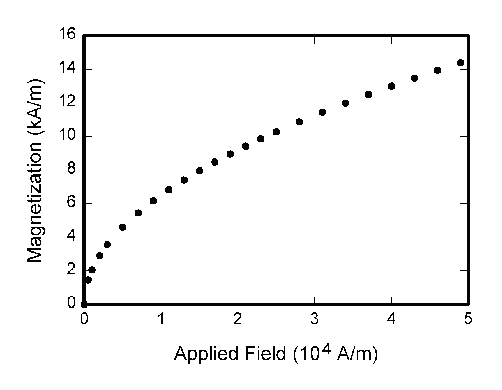
\includegraphics[scale=1]{field1.eps}
        \caption{Podajte kratko razlago slike.} \label{slika}
    \end{center}
\end{figure}

\section{Oddaja prispevka}

Prispevek oddajte v elektronski obliki preko formularja na spletni strani \cite{ERK}. Sprejemamo prispevke v formatu pdf (brez nastavljenih zaščitnih gesel) ali Microsoft Word. Pred oddajo prispevka prosimo preverite dodatne informacije za avtorje, ki so na spletnih straneh. 

Formular za elektronsko oddajo prispevkov bo aktiviran v juniju, rok za oddajo je \textbf{13. julij 2014}. Avtorje bomo obvestili o izboru konec avgusta.

\small
\begin{thebibliography}{1}

\bibitem{ERK} ERK, http://www.ieee.si/erk/index.html 
\bibitem{Zbornik} B. Zajc, A. Trost: Zbornik triindvajsete mednarodne Elektrotehniške in računalniške konference ERK 2014, 22. - 24. September 2014, Portorož, Slovenija

\end{thebibliography}

\end{document}
